\documentclass[15pt, a4paper, oneside]{report}
%%%%%%%%%%%%%%%%%%%                LIBRARY %%%%%%%%%%%%%%%%%%%%%%%%%
\usepackage[utf8]{inputenc}
\usepackage{afterpage}
\usepackage{lastpage}
\usepackage{xcolor}
\usepackage{listings}
\usepackage{sectsty}
\usepackage{geometry}

\usepackage[T1]{fontenc}
\usepackage{titlesec}
\usepackage[pdftex]{graphicx} %PDF Graphik
\usepackage[pdftex]{hyperref} %PDF Referenzen
\usepackage{times}
\usepackage[export]{adjustbox}
%\usepackage{float}
%\usepackage{floatflt}
\usepackage{amsmath}
\usepackage{amssymb}
\usepackage{amsthm}
%\usepackage[ngerman,english]{babel}
\usepackage[right]{eurosym}
\usepackage{color} %red, green, blue, yellow, cyan, magenta, black, white
\usepackage{ulem}
\usepackage{longtable}
\usepackage{multirow}
\usepackage[shortlabels]{enumitem} % Itemize with letters package
\usepackage{ltxtable}
\usepackage{ragged2e, tabularx, tabulary}
\newcolumntype{Y}{>{\RaggedRight\arraybackslash}X}
\usepackage{cancel}
\usepackage{wrapfig}
\usepackage{hyperref}
\hypersetup{
    pdfborderstyle={/S/U/W 1}, % underline links instead of boxes
    colorlinks=true,
    linkcolor=blue,
    filecolor=magenta,      
    urlcolor=blue,
}

\definecolor{mygreen}{RGB}{28,172,0} % color values Red, Green, Blue
\definecolor{mylilas}{RGB}{170,55,241}





\geometry{
 a4paper,
 total={170mm,257mm},
 left=5mm, right = 5mm,
 top=20mm, bottom = 20mm
 }
\usepackage{tocloft}
\renewcommand\cftsecfont{\Large}
\renewcommand\cftsecpagefont{\Large}
\renewcommand\cftsecafterpnum{\vskip15pt}
\renewcommand\cftsubsecafterpnum{\vskip5pt}
% Title formating


\usepackage{fancyhdr}

\pagestyle{fancy}
\fancyhf{}
\fancyhead[LE,RO]{Embedded Computing Lab\\Prof. Markus Pfeil }
\fancyhead[RE,LO]{ ET1 Control }
\fancyfoot[CE,CO]{\thepage}
\fancyfoot[LE,RO]{
\includegraphics[width=0.15\textwidth]{./rwu}}
\fancyfoot[RE,LO]{\textbf{Task 5}}

\renewcommand{\headrulewidth}{2pt}
\renewcommand{\footrulewidth}{2pt}

\lstset{language=Python,%
    %basicstyle=\color{red},
    breaklines=false,%
    morekeywords={matlab2tikz},
    keywordstyle=\color{blue},%
    morekeywords=[2]{1}, keywordstyle=[2]{\color{black}},
    identifierstyle=\color{black},%
    stringstyle=\color{mylilas},
    commentstyle=\color{mygreen},%
    showstringspaces=false,%without this there will be a symbol in the places where there is a space
    numbers=left,%
    numberstyle={\tiny \color{black}},% size of the numbers
    numbersep=9pt, % this defines how far the numbers are from the text
    emph=[1]{for,end,break},emphstyle=[1]\color{red}, %some words to emphasise
    %emph=[2]{word1,word2}, emphstyle=[2]{style},    
}


\urlstyle{same}

\begin{document}



\newpage


\normalfont

\vspace*{5mm}

\section*{\Large Task 5: Distance Measurement and Plotting}

\vspace{2mm}
    \Large

    

\subsection*{\Large Solution}

\subsection*{\Large Distance Measurement Using Ultrasonic Sensor}
    \begin{itemize}
        \item  To measure the distance on the ET1 device, we use the two-way distance measurement technique with ultrasonic sensor.\\
        \item This means that we send out a pulsed sonar wave which reflects back on hitting an obstacle.
        Using the time and speed of sound, the distance of object from Robot can be measured.\\
        Preferably use the GPIOzero Library in this case.
        
\begin{lstlisting}[language=Python]

# Pin for Ultrasonic Sensor
trigger = 25
echo = 27
    
sensor = DistanceSensor(echo = 27, trigger = 25)

for i in range(20):
    print(str(round(sensor.distance*100, 2)) + 'cm') # %2d
    led.on()
    time.sleep(1)

\end{lstlisting}
\end{itemize}
\newpage

    
    \subsection*{\Large Accuracies and Dependencies}
\vspace{5mm}
    \begin{itemize}
        \item For optimal measurements, object positioned at right angles to the ultrasonic sensor.
        
        If the angle to the surface object is not 90°, the returning sound can be deflected away from the transducer, and it will no longer be detectable. \\
        The amplitude of the reflected ultrasonic signal must be high enough to allow reliable measurements. 
        \vspace{3mm}
        
        \item Since the Ultrasonic sensor disperses horizontally and vertically by about 25° and 13° respectively, it is key that the object used is not too far off but directly in front of the robot.
        \vspace{3mm}
        
        \item Experiments show that the distance range from obstacle for measurement should be within 1m.
        \vspace{3mm}
        
        \item Color is of no consequence and they can detect solids or liquids.
        \vspace{3mm}
        
        \item Surface properties also have no effect on detection reliability.\\
        It does not matter if the surface is rough, smooth, high gloss, transparent, dirty, wet, or dry – a high-quality ultrasonic sensor delivers precise results.

\end{itemize}
\newpage

    
    

\subsection*{\Large Distance Measurement for changing Speed Setting}
    \begin{itemize}
        \item  Measuring distances with the robot is quite simple. But, what happens if the speed is changed?\\
        
        At higher speeds, number of measured distance points per time decrease and as expected, same distance would be covered in shorter time period.
       
       Let's see a case for two different speed settings: 28 and 50.\\ 
       This is done by changing the PWM values for each measurement.
            
\begin{lstlisting}[language=Python]

# Speed setting: 28, 50 \\Slower speeds for better measurement
SpeedArr = [28, 50];
    
def Robot_Meas(p):
    start = time.time()

    # threshold distance = 20cm, Max.distance = 1m
    while round(sensor.distance * 100, 2) > 20 and < 100:
        Time_Dist_Meas(start)
        Robot_Drive(p)  # Robot moves at given speed - 'p'

    end = time.time()
    Robot_STOP()
    
    # Loop using Speed Settings
for i in SpeedArr:
    filename = str(str(i) + '.txt') # file name using speed 
    print(filename)
    x = open(filename, 'w')
    TitleName(i)                # Title of text file

    led.on()
    Robot_Meas(i)
    led.off()

    # Manually return robot to original position
    time.sleep(5)  # Begin after 5s
    x.close()  # Close the file

\end{lstlisting}

\item The use of a certain distance ranges is to maintain accuracy in measurement and prevent crashing the robot.

\end{itemize}

\newpage

\begin{center}

    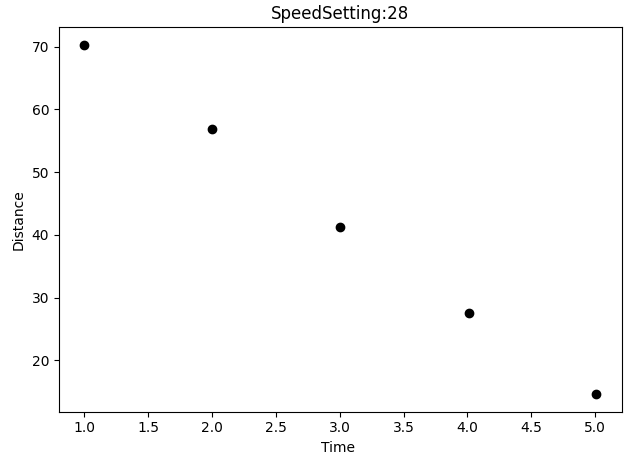
\includegraphics[width=0.7\textwidth]{./Speed_28}
    
    \vspace{1.5cm}
    
    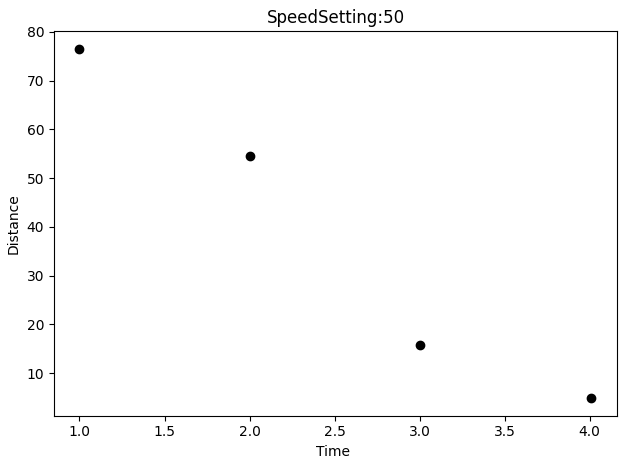
\includegraphics[width=0.7\textwidth]{./Speed_50}
\end{center}


  
\vspace{1cm}


\end{document}